\documentclass[BoSSSForSolvingConservationLaws.tex]{subfiles}

\begin{document}
For solving a system of linear equations demonstrated as below we need linear solvers.
\[
M \vec{x}= rhs
\]
Our matrix $M$ is a sparse matrix therefore we call the solvers \emph{sparse solvers}. $\vec{x}$ is array of unknowns and $rhs$ is an array representing the right hand side. $rhs$ is sum of right hand side of the equation, RHS (if it exists) minus the affine offset of the spatial differential operator. For solving this system of equations direct or iterative solvers may be used.

\subsection*{Implementation in BoSSS}
Sparse solvers in BoSSS implement the interface \emph{ISparseSolver}\coderm{ilPSP.LinSolvers.ISparseSolver}. All sparse solvers have two methods $DefineMatrix()$\coderm{ilPSP.LinSolvers.ISparseSolver.DefineMatrix(...)} and $Solve()$\coderm{ilPSP.LinSolvers.ISparseSolver.Solve(...)} that have different implementations for different solvers. The first method is used to define the matrix $M$ (which is a \emph{sparse matrix}) for the solver. The second one is used to solve the system by taking $\vec{x}$ and $rhs$ which are both list of doubles. By calling the method solve unknowns are calculated and \emph{solver result}\coderm{ilPSP.LinSolvers.SolverResult} is returned. Solver result  contains information about the solved system like run time, number of iterations, if the iterative solver is converged and the convergence type (absolute, relative or other). As an example you can look at a linear solver\coderm{BoSSS.Solution.Solver.LinearSolver} used for solving Poisson equation.\\
There is also an extended version of sparse solvers, \emph{ISparseSolverExt}\coderm{ilPSP.LinSolvers.ISparseSolverExt} used for solving the system in the following form
\[
\Big(diag(d0,d1,...)+M \Big) \vec{x}= rhs
\]
This version is used for time dependent equations (look at section \ref{sec:Timediscretization}, \nameref{sec:Timediscretization}). The method solve\coderm{ilPSP.LinSolvers.ISparseSolverExt.Solve(...)} of the extended version takes also the list of double values $d_0,...,d_n$. For the extended version there is a method $GetMatrix()$ that returns matrix $M$ if required.\\
There are some available solvers used until now; like PARDISO solver\coderm{ilPSP.LinSolvers.PARDISO.PARDISOSolver} which is a direct solver and some iterative solvers from Aztec\coderm{ilPSP.LinSolvers.Aztec.Solver} and HYPRE\coderm{ilPSP.LinSolvers.HYPRE.Solver} libraries. \emph{monkey}\coderm{ilPSP.LinSolvers.monkey.Solver} library is the implemented library in BoSSS.
\subsubsection*{Creating sparse solvers}
There are two types of preconditioning for iterative solvers considered as explicit\coderm{ilPSP.LinSolvers.IExplicitPrecond} and implicit\coderm{ilPSP.LinSolvers.IImplicitPrecond} in BoSSS. Both explicit and implicit preconditioners are in fact sparse solvers themselves. The explicit preconditioning is the one performed before starting the iterative procedure of an iterative sparse solver which is called \emph{nested solver}\coderm{ilPSP.LinSolvers.IExplicitPrecond.NestedSolver}. An Explicit preconditioner is supposed to change the sparse matrix $M$ (in its define matrix method) and hand it over to (by calling the define matrix method of) the nested solver. In its solve method it should perform the same changes to the $rhs$ and call the solve method of the nested solver. Local block elimination\coderm{ilPSP.LinSolvers.GenPrecond.LocalBlockElimination} is an example of explicit preconditioning.\\
Some sparse solvers support\coderm{ilPSP.LinSolvers.IImplicitPrecondSupport} implicit preconditioning which means that they can use other solvers as preconditioners. For these solvers there is a collection\coderm{ilPSP.LinSolvers.IImplicitPrecondSupport.SupportedPrecond} of supported implicit preconditioners available. An implicit preconditioner that is called \emph{nested preconditioner}\coderm{ilPSP.LinSolvers.IImplicitPrecondSupport.NestedPrecond} is performed within each iteration of the sparse solver. An example from HYPRE library of such solvers are PCG\coderm{ilPSP.LinSolvers.HYPRE.PCG} or GMRES\coderm{ilPSP.LinSolvers.HYPRE.GMRES} that can take Euclid\coderm{ilPSP.LinSolvers.HYPRE.Euclid} or ParaSails\coderm{ilPSP.LinSolvers.HYPRE.ParaSails} or BoomerAMG\coderm{ilPSP.LinSolvers.HYPRE.BoomerAMG} as nested preconditioner.\\
We can imagine creating a solver in general form of ''explicit preconditioner+sparse solver+ implicit preconditioner''. Here the solver would be the explicit preconditioner which has a nested solver and the nested solver has a nested preconditioner. There are some properties specific to each iterative sparse solver that can be adjusted (otherwise they may have default values); like maximum iterations, convergence type, tolerance (threshold for convergence), device type (CPU or GPU for monkey library) and so on. The easiest way of creating an appropriate solver including preconditioning is probably using a BoSSS control file (if it exists) and specifying the name of libraries, type of solvers and some specifications. The information is obtained\coderm{BoSSS.Solution.Control.AppControl.Solver.GetExtProperty(...)} as \emph{solver configurations}\coderm{BoSSS.Solution.Control.AppControl.SparseSolvers.SolverConfigurations}. This \emph{configuration}\coderm{ilPSP.LinSolvers.Configuration} is used by \emph{solver factory}\coderm{ilPSP.LinSolvers.SolverFactory} to create the desired solver. To see an example look at (method create equations and solvers of) ipPoisson;  one of example applications of BoSSS in layer $4$.

\subsubsection*{Sparse matrix}
\label{sec:MsrMatrix}
The sparse matrix $M$ that is used with sparse solvers is referred to as \emph{ISparseMatrix}\coderm{ilPSP.LinSolvers.ISparseMatrix} in BoSSS. It defines the minimum requirements for a sparse matrix data structure. \emph{MsrMatrix}\coderm{ilPSP.LinSolvers.MsrMatrix} ('M'utuable 'S'parse 'R'ow matrix) is the implemented sparse matrix. For creating this matrix we need to know row partition, number of columns, number of rows per block and number of columns per block. Here each block corresponds to one cell. The block's row and column sizes are the ''maximum total number of coordinates per cell'' of the codomain and domain mappings (see section \ref{sec:CoordinateMapping} \nameref{sec:CoordinateMapping}). Partitioning means distributing a vector or matrix among processors. A \emph{partition}\coderm{ilPSP.LinSolvers.Partition} can be created by knowing the required local size which is (here for row partitioning) the ''number of coordinates in locally updated cells'' (\emph{NUpdate}\coderm{BoSSS.Foundation.UnsetteledCoordinateMapping.NUpdate}) of codomain mapping. Number of columns is equal to ''total number of coordinates in all processors'' (\emph{GlobalCount}\coderm{BoSSS.Foundation.UnsetteledCoordinateMapping.GlobalCount}) of the domain mapping.\\
\begin{figure}[h]
\begin{center}
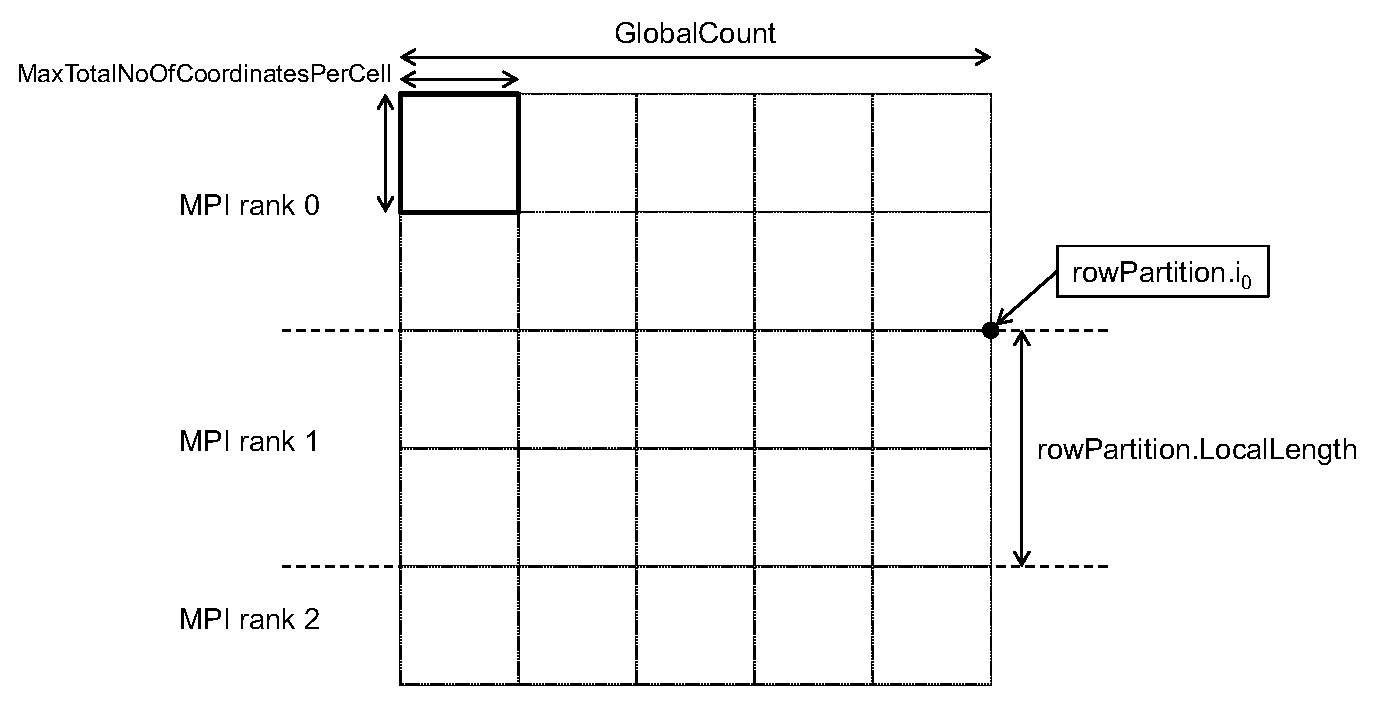
\includegraphics[width=12cm]{Figures/MsrMatrix}
\end{center}
\caption{Structure of MsrMatrix.}
\end{figure}
\emph{RefMatrix}\coderm{ilPSP.LinSolvers.monkey.CPU.RefMatrix} (Reference Matrix) is a sparse matrix created from an MsrMatrix by partitioning also its columns.

\end{document} 